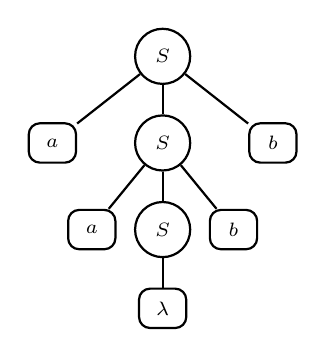
\begin{tikzpicture}[
    node distance=0.8cm,
    every node/.style={font=\scriptsize},
    nt/.style={draw, circle, thick, minimum size=7mm},
    t/.style={draw, rounded corners, thick, minimum width=6mm, minimum height=5mm}
]
    \node<5->[nt] (S) at (0,0) {$S$};
    \node<6->[t] (a1) at (-1.4,-1.1) {$a$};
    \node<6->[nt] (S2) at (0,-1.1) {$S$};
    \node<6->[t] (b1) at (1.4,-1.1) {$b$};

    \node<7->[t] (a2) at (-0.9,-2.2) {$a$};
    \node<7->[nt] (S3) at (0,-2.2) {$S$};
    \node<7->[t] (b2) at (0.9,-2.2) {$b$};

    \node<8->[t] (eps) at (0,-3.2) {$\lambda$};

    \draw<6->[thick] (S) -- (a1);
    \draw<6->[thick] (S) -- (S2);
    \draw<6->[thick] (S) -- (b1);

    \draw<7->[thick] (S2) -- (a2);
    \draw<7->[thick] (S2) -- (S3);
    \draw<7->[thick] (S2) -- (b2);

    \draw<8->[thick] (S3) -- (eps);
\end{tikzpicture}
